% ----------------------------------------------------------------- %
%             The Speech Signal Processing Toolkit (SPTK)           %
%             developed by SPTK Working Group                       %
%             http://sp-tk.sourceforge.net/                         %
% ----------------------------------------------------------------- %
%                                                                   %
%  Copyright (c) 1984-2007  Tokyo Institute of Technology           %
%                           Interdisciplinary Graduate School of    %
%                           Science and Engineering                 %
%                                                                   %
%                1996-2016  Nagoya Institute of Technology          %
%                           Department of Computer Science          %
%                                                                   %
% All rights reserved.                                              %
%                                                                   %
% Redistribution and use in source and binary forms, with or        %
% without modification, are permitted provided that the following   %
% conditions are met:                                               %
%                                                                   %
% - Redistributions of source code must retain the above copyright  %
%   notice, this list of conditions and the following disclaimer.   %
% - Redistributions in binary form must reproduce the above         %
%   copyright notice, this list of conditions and the following     %
%   disclaimer in the documentation and/or other materials provided %
%   with the distribution.                                          %
% - Neither the name of the SPTK working group nor the names of its %
%   contributors may be used to endorse or promote products derived %
%   from this software without specific prior written permission.   %
%                                                                   %
% THIS SOFTWARE IS PROVIDED BY THE COPYRIGHT HOLDERS AND            %
% CONTRIBUTORS "AS IS" AND ANY EXPRESS OR IMPLIED WARRANTIES,       %
% INCLUDING, BUT NOT LIMITED TO, THE IMPLIED WARRANTIES OF          %
% MERCHANTABILITY AND FITNESS FOR A PARTICULAR PURPOSE ARE          %
% DISCLAIMED. IN NO EVENT SHALL THE COPYRIGHT OWNER OR CONTRIBUTORS %
% BE LIABLE FOR ANY DIRECT, INDIRECT, INCIDENTAL, SPECIAL,          %
% EXEMPLARY, OR CONSEQUENTIAL DAMAGES (INCLUDING, BUT NOT LIMITED   %
% TO, PROCUREMENT OF SUBSTITUTE GOODS OR SERVICES; LOSS OF USE,     %
% DATA, OR PROFITS; OR BUSINESS INTERRUPTION) HOWEVER CAUSED AND ON %
% ANY THEORY OF LIABILITY, WHETHER IN CONTRACT, STRICT LIABILITY,   %
% OR TORT (INCLUDING NEGLIGENCE OR OTHERWISE) ARISING IN ANY WAY    %
% OUT OF THE USE OF THIS SOFTWARE, EVEN IF ADVISED OF THE           %
% POSSIBILITY OF SUCH DAMAGE.                                       %
% ----------------------------------------------------------------- %
\hypertarget{dfs}{}
\name{dfs}{digital filter in standard form}{digital filter}

\begin{synopsis}
\item[dfs] [ --a $K$ $a(1)$ $\dots$ $a(M)$ ] 
	   [ --b $b(0)$ $b(1)$ $\dots$ $b(N)$ ] 
	   [ --p {\em pfile} ] [ --z {\em zfile} ]
\item[\ ~~~] [ {\em infile} ]
\end{synopsis}

\begin{qsection}{DESCRIPTION}
{\em dfs} filters data from {\em infile} (or standard output) 
using a digital filter in standard form, 
sending the result to standard output.
  The filter transfer function is given by:
\begin{displaymath}
  H(z) 
  = 
  K\frac{\displaystyle{\sum_{n=0}^{N}{b(n)z^{-n}}}}{1+\displaystyle{\sum_{m=1}^{M}{a(m)z^{-m}}}}
\end{displaymath}
\par
Both input and output files are in float format.
\end{qsection}

\begin{options}
	\argm{a}{K \; a(1) \dots a(M)}{denominator coefficients,
                       where $K$ is the gain of the transfer function.}{N/A}
	\argm{b}{b(0) \; b(1) \dots b(N)}{numerator coefficients}
		{N/A}
	\argm{p}{pfile}{denominator coefficients file in float format
                as follows\\
		\hspace*{2ex}$K, a(1), \ldots, a(M)$\\[-1ex]}{NULL}
	\argm{z}{zfile}{numerator coefficients file in float format
                as follows\\
		\hspace*{2ex}$b(0), b(1), \ldots, b(N)$\\[-1ex]}{NULL}
	\desc{If the option {\bf --a} and {\bf --p} are not specified, then
          both $K$ and the denominator are set to 1. On the other
          hand, if the option {\bf --b} and {\bf --z} are not specified,
          then the numerator is set to 1.}
\end{options}

\begin{qsection}{EXAMPLE}
In order to visualize the impulse response of the following transfer
 function
\begin{displaymath}
  H(z)=\frac{1+2z^{-1}+z^{-2}}{1+0.9z^{-1}}
\end{displaymath}
the command below can be used
\begin{quote}
 \verb!impulse | dfs -a 1 0.9 -b 1 2 1 | dmp +f!
\end{quote}
\par
For visualizing the frequency response plot of the digital filter,
whose coefficients are defined in float format by the files
{\em data.p, data.z}, then the following command can be used.
\begin{quote}
 \verb!impulse | dfs -p data.p -z data.z | spec | fdrw | xgr!
\end{quote}
\begin{center}
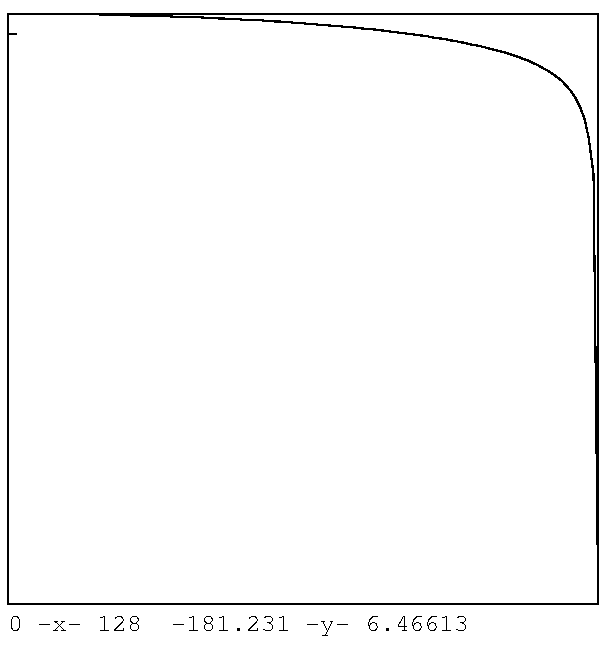
\includegraphics[width=6cm]{fig/dfs.pdf}
\end{center}
The files {\em data.p} and {\em data.z} can be obtained
through the {\em x2x} command.
\end{qsection}
